\begin{figure}
 \centering  % this centres figure in column
  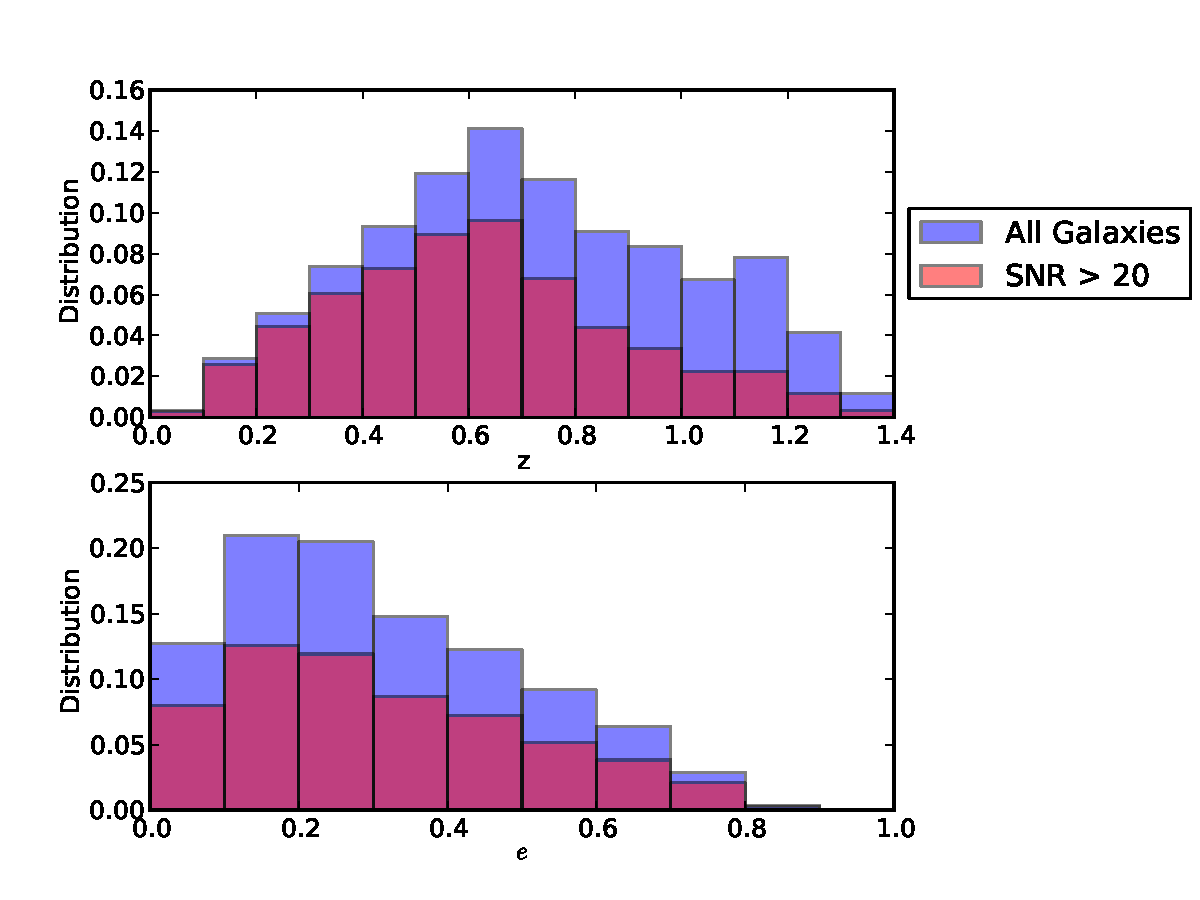
\includegraphics[width=0.45\textwidth]{fig/Out_hist_v2_truth.pdf} 
  \caption{Distributions of redshift (top panel) and intrinsic ellipticity (bottom panel) in the CSTEP simulation.
The full galaxy sample ($\approx140,000$) is shown in blue, the objects with SNR $>$ 20 ($\approx85,000$) is shown in magenta. \green{use larger labels; especially the x axis labels are hard to read; intrinsic size and Sersic index might be interesting to plot as well}}
\label{fig:Galprop}
\end{figure}

The image simulations used in the CSTEP project were designed to 
replicate the properties of the co-added data of final depth that will be taken by the 
Dark Energy Survey. The Dark Energy survey is an optical survey of
5000 deg$^2$ of the southern sky, that will image around 300 million
galaxies in five filters (g,r,i,z and Y) \citep{Klaus}. To test the DES
data management system and software pipelines, detailed image simulations were created \citep{DESsim}. Each simulated image used in CSTEP models the DES focal plane,
with 62 CCDs each of which is 2K $\times$ 4K pixels (0.27''/pixel). Star and galaxy objects are
rendered by drawing random samples of
photons from the theoretical light profile of the source convolved 
by the PSF.

The CSTEP simulated images are based on an N-body simulation with a realistic mock galaxy catalog.
The parent N-body simulations used by ADDGALS are the ``Carmen'' Las Damas \citep{LasDamas}
N-body simulation box (1$h^{-3}$Gpc$^3$) with a fiducial $\Lambda$CDM cosmology ($\Omega_M=0.25$, $\sigma_8 = 0.8$, at $z< 1.35$). In each DES focal plane around $140,000$ galaxy objects are
present. Mock galaxy catalogs were
created with the ADDGALS  method, which reproduces observed properties
of galaxies including clustering, luminosities, and colors. 

The simulated galaxy images are designed to have properties similar to
the galaxies that DES will observe by combining a mock
catalog with empirical data from the HST/GEMS catalog for galaxies
with magnitude r $ > $ 23, and from the Sloan Digital Sky Survey for
galaxies with magnitude r $ < $ 23. The distributions of galaxy
properties in the simulation are shown in Figure \ref{fig:Galprop}. 
The galaxy objects are created with Sersic profiles with an
index that ranges from 0.5 to 5.

 The CSTEP simulated images contain a constant
PSF, which eliminates the technical challenge of determining the best
way to model a varying PSF \citep[see][for a simulation challenge for PSF reconstruction]{GREAT10star}. For CSTEP there are two
branches in the image simulation sets, one with a circular
Gaussian PSF and one with an elliptical Gaussian PSF. 
The elliptical Gaussian PSF has $ \epsilon =
0.03 $. The simulated seeing FWHM of $ 0.7 - 0.9 $ arcsec matches the expected seeing in final DES data for different levels of atmospheric turbulence.
A summary of the PSF image properties is shown in the upper part of Table \ref{table:tab2}. 
For each PSF there are 8 focal plane images that contain constant
shear for $\gamma = 0.0$ to $\gamma = 0.15$ in both
$\gamma_1$ and $\gamma_2$, as described in the lower part of Table \ref{table:tab2}.  

\green{you never discuss the additive bias later; I think one good way of thinking about it is a leakage of PSF ellipticity into the shear estimate. Is $c$ much different for the round and elliptical PSF data sets?}


\begin{table}
\centering
\begin{centering}
\begin{tabular}{ccc}
\hline
PSF Number & Type & Seeing  \\
\hline
1 & circular Gaussian & 0.7 \\
2 & circular Gaussian & 0.8 \\
3 & circular Gaussian & 0.9 \\
4 & elliptical Gaussian & 0.75 \\
5 & elliptical Gaussian & 0.8  \\
6 & elliptical Gaussian & 0.9  \\
\hline
\hline
Shear Number & $ \gamma_1 $ & $ \gamma_2 $  \\
\hline
1 &  0.0 & 0.03 \\
2 &  0.0 & 0.06 \\
3 &  0.0 & 0.09 \\
4 &  0.0 & 0.15 \\
5 &  0.03 & 0.0 \\
6 &  0.06 & 0.0 \\
7 &  0.09 & 0.0 \\
8 &  0.15 & 0.0 \\
\hline
\end{tabular}
\end{centering}
\caption{ Summary of the PSF and shear sets for the CSTEP simulated images. }
\label{table:tab2}
\end{table}
